\addcontentsline{toc}{chapter}{Anhang} %sorgt für eintrag ins inhaltsverzeichnis
\chapter{Ergänzungen zur Forschungsfrage eins} \label{appendixFF1}
In diesem Teil des Anhangs sind Ergänzungen zur Forschungsfrage eins des Kapitels \vref{ff1} beschrieben.

\section{Anforderungsdokument}\label{appendixAnforderung}

Ein Anforderungskatalog hat bestimmte Anforderungen, die an den Katalog gestellt werden. Neben der Forderung nach Einhaltung der Qualitätskriterien, definiert nach dem ISO-Standard 9000/9001, sind noch folgende Forderungen in der Literatur beschrieben: \autocite[sig.][S.\,34]{partsch_requirements-engineering_2010}

\begin{itemize}
	\item vollständig (inhaltlich – d.\,h., alle Anforderungen sind erfasst –, formal, Norm-konform)
	\item konsistent (keine Widersprüche zwischen den Bestandteilen des Dokuments,
	insbesondere keine Konflikte zwischen verschiedenen Anforderungen)
	\item lokal änderbar (Änderungen an einer Stelle sollten keine Einflüsse auf Konsistenz und Vollständigkeit des Gesamtdokuments haben)
	\item verfolgbar (ursprüngliche Stakeholderwünsche und Zusammenhänge zwischen
	Anforderungen sind leicht zu finden)
	\item klar strukturiert
	\item umfangsmäßig angemessen
	\item sortierbar/projizierbar (nach verschiedenen Kriterien, für verschiedene Stakeholder).
\end{itemize}

Die folgende Aufzählung beschreibt eine Vorlage für das Anforderungsdokument nach Quelle: Sie nutzt die Hilfsmittelsammlung \enquote{Volere}. Diese bietet im Themenbereich \enquote{requirements engineering} kostenpflichtig Dokumentenvorlagen an. Die beiden Bekanntesten sind die hier gezeigte \enquote{Volere Requirements Specification Template} und das kostenlose \enquote{Volere Atomic Requirement Template}, das umgangssprachlich \enquote{Snow Card} genannt wird. Die \enquote{Snow Card} (\vref{abb:volereSnowCard}) ist eine Karteikarte, die benutzt wird, um eine vollständige Aufnahme aller Informationen einer einzelnen Anforderung zu gewährleisten.\autocite[vgl.][]{VolereSnowCard} 

\begin{figure}[H]
	\centering
	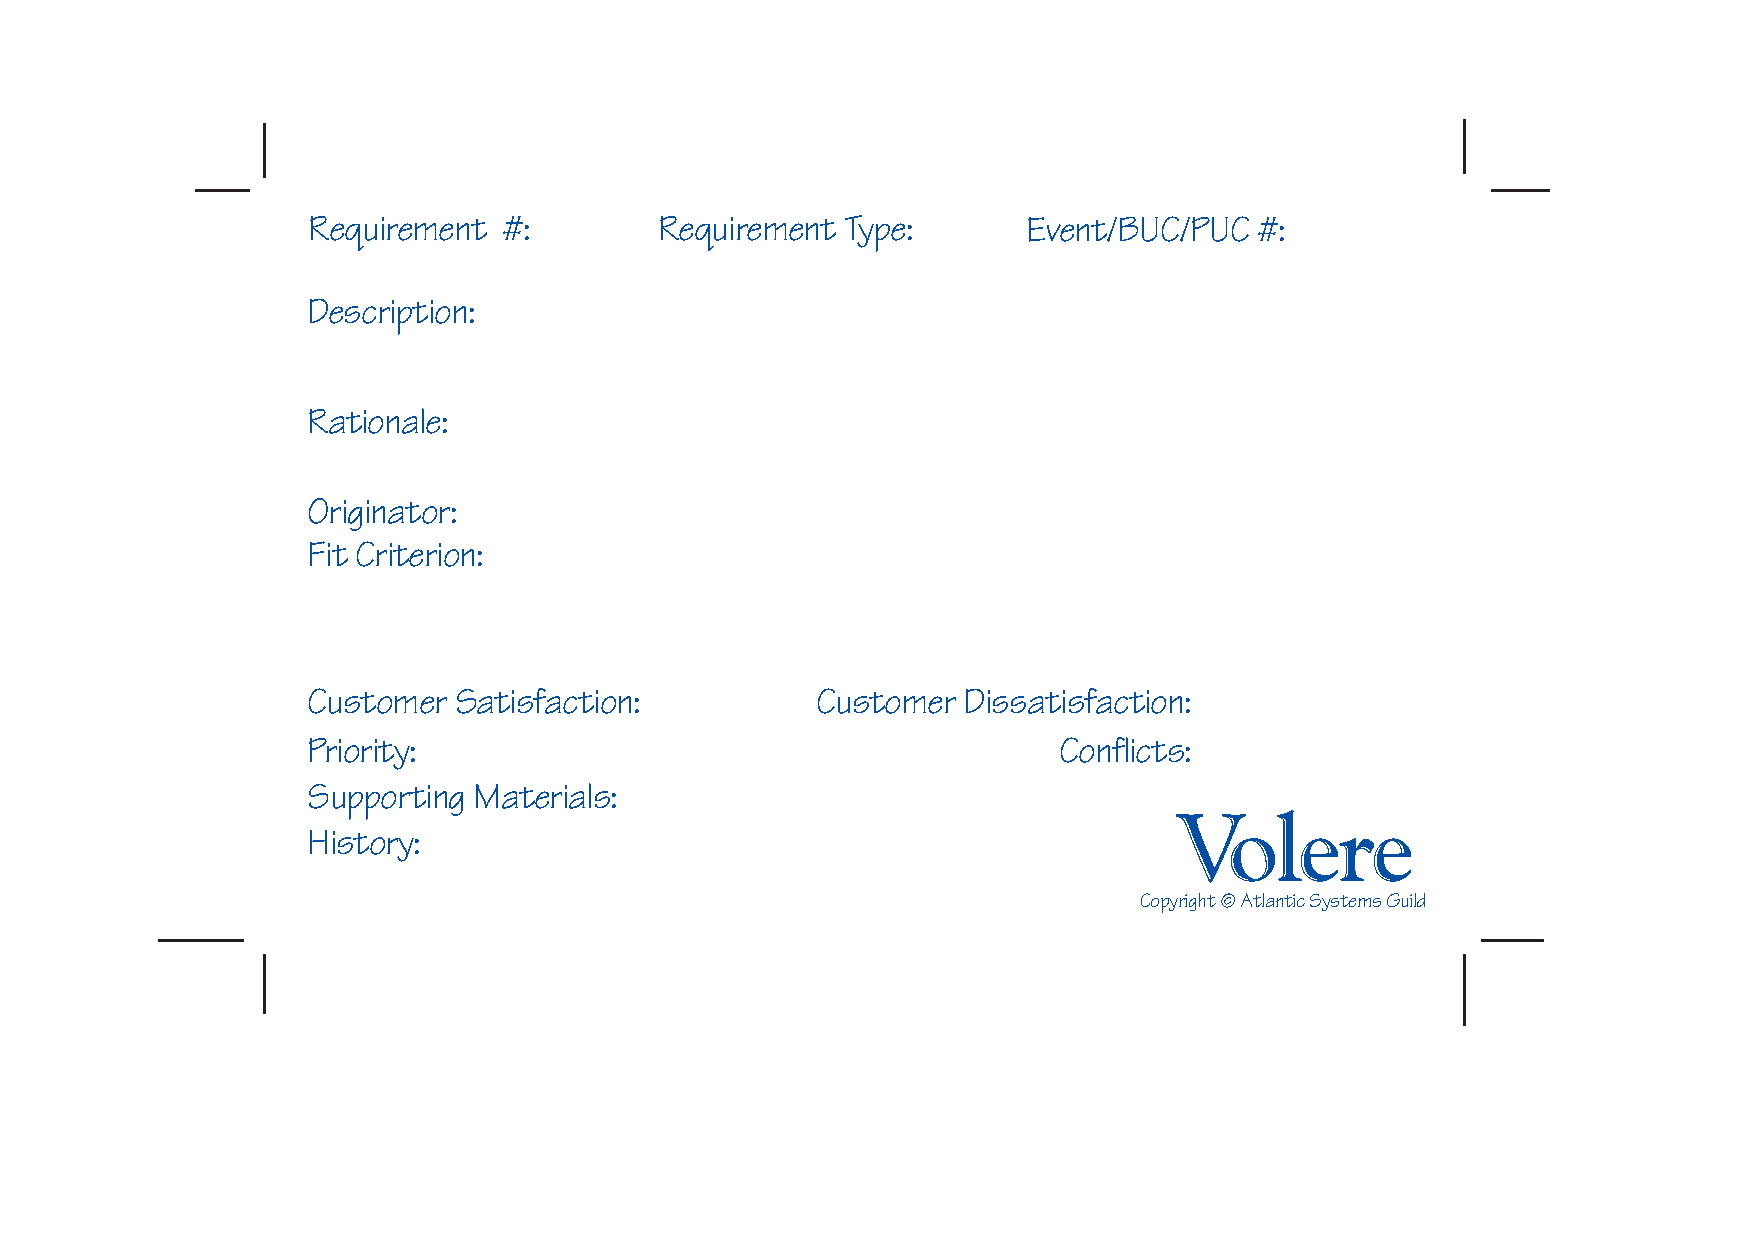
\includegraphics[scale=0.6]{img/snowcard.pdf}
	\caption{Volere Snow Card}
	{\footnotesize Quelle: \cite{VolereSnowCard}}
	\label{abb:volereSnowCard}
	%		{\scriptsize \textit{Alle Rechte, einschließlich der Vervielfältigung, Veröffentlichung, Bearbeitung und Übersetzung bleiben der SV Informatik GmbH vorbehalten.}}
\end{figure}

Die folgende Liste wurde in Anlehnung an die Quelle \cite{VolereRequirmentsSpecTemplate} erstellt.

\begin{minipage}{\linewidth}
	\begin{itemize}\label{abb:volereReqSpec}
		\item Projekt-Treiber
		\begin{enumerate}
			\item Zweck des Projekts
			\item Auftraggeber, Kunde und andere Stakeholder
			\item Nutzer des Produkts
		\end{enumerate}
		\item Projekt-Randbedingungen
		\begin{enumerate}
			\item Einschränkungen
			\item Namenskonventionen und Definitionen
			\item Relevante Fakten und Annahmen
		\end{enumerate}
		\item Funktionale Anforderungen
		\begin{enumerate}
			\item Arbeitsrahmen
			\item Systemgrenzen
			\item Funktionale und Daten-Anforderungen
		\end{enumerate}
		\item Nicht-funktionale Anforderungen
		\begin{enumerate}
			\item Look-and-Feel-Anforderungen
			\item Usability-Anforderungen
			\item Performanz-Anforderungen
			\item Operationale und Umfeld-Anforderungen
			\item Wartungs- und Unterstützungsanforderungen
			\item Sicherheitsanforderungen
			\item Kulturelle und politische Anforderungen
			\item Rechtliche Anforderungen
		\end{enumerate}
		\item Projekt-Aspekte
		\begin{enumerate}
			\item Offene Punkte
			\item Standardlösungen
			\item Neu aufgetretene Probleme
			\item Installationsaufgaben
			\item Migrationstätigkeiten
			\item Risiken
			\item Kosten
			\item Nutzerdokumentation
			\item Zurückgestellte Anforderungen
			\item Lösungsideen
		\end{enumerate}
	\end{itemize}
\end{minipage}

\clearpage
\begin{figure}[H]
	\centering
	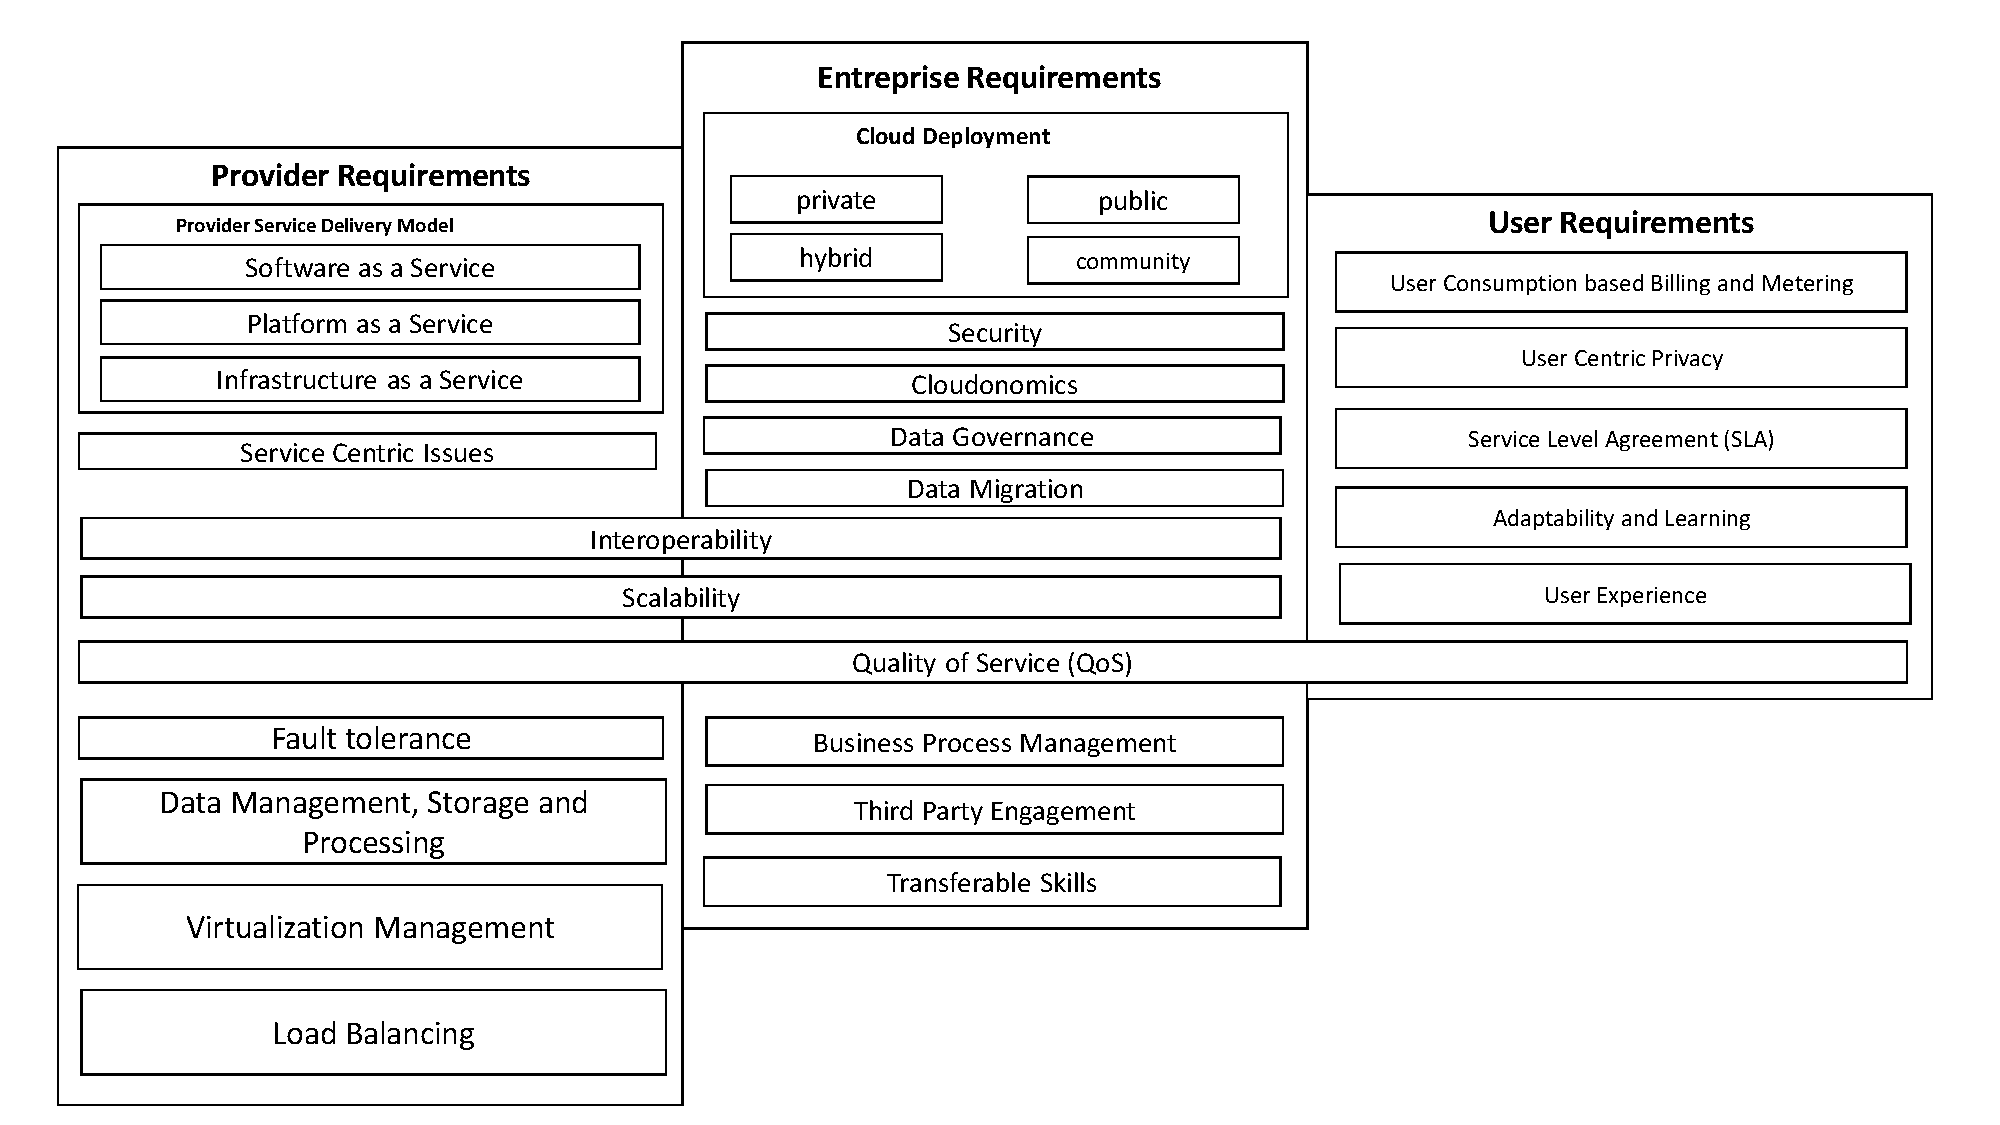
\includegraphics[scale=0.50, angle=90]{img/cloudreq.pdf}
	\caption{Ebenen der \enquote{Cloud}-Anforderungsanalyse}
	{\footnotesize Quelle: in Anlehnung an \cite{rimal_architectural_2011}}
	\label{abb:cloudreq}
	%		{\scriptsize \textit{Alle Rechte, einschließlich der Vervielfältigung, Veröffentlichung, Bearbeitung und Übersetzung bleiben der SV Informatik GmbH vorbehalten.}}
\end{figure}

\clearpage
\section{Statistiken zum Themengebiet \ac{Cloud-C}}

\begin{figure}[H]
	\centering
	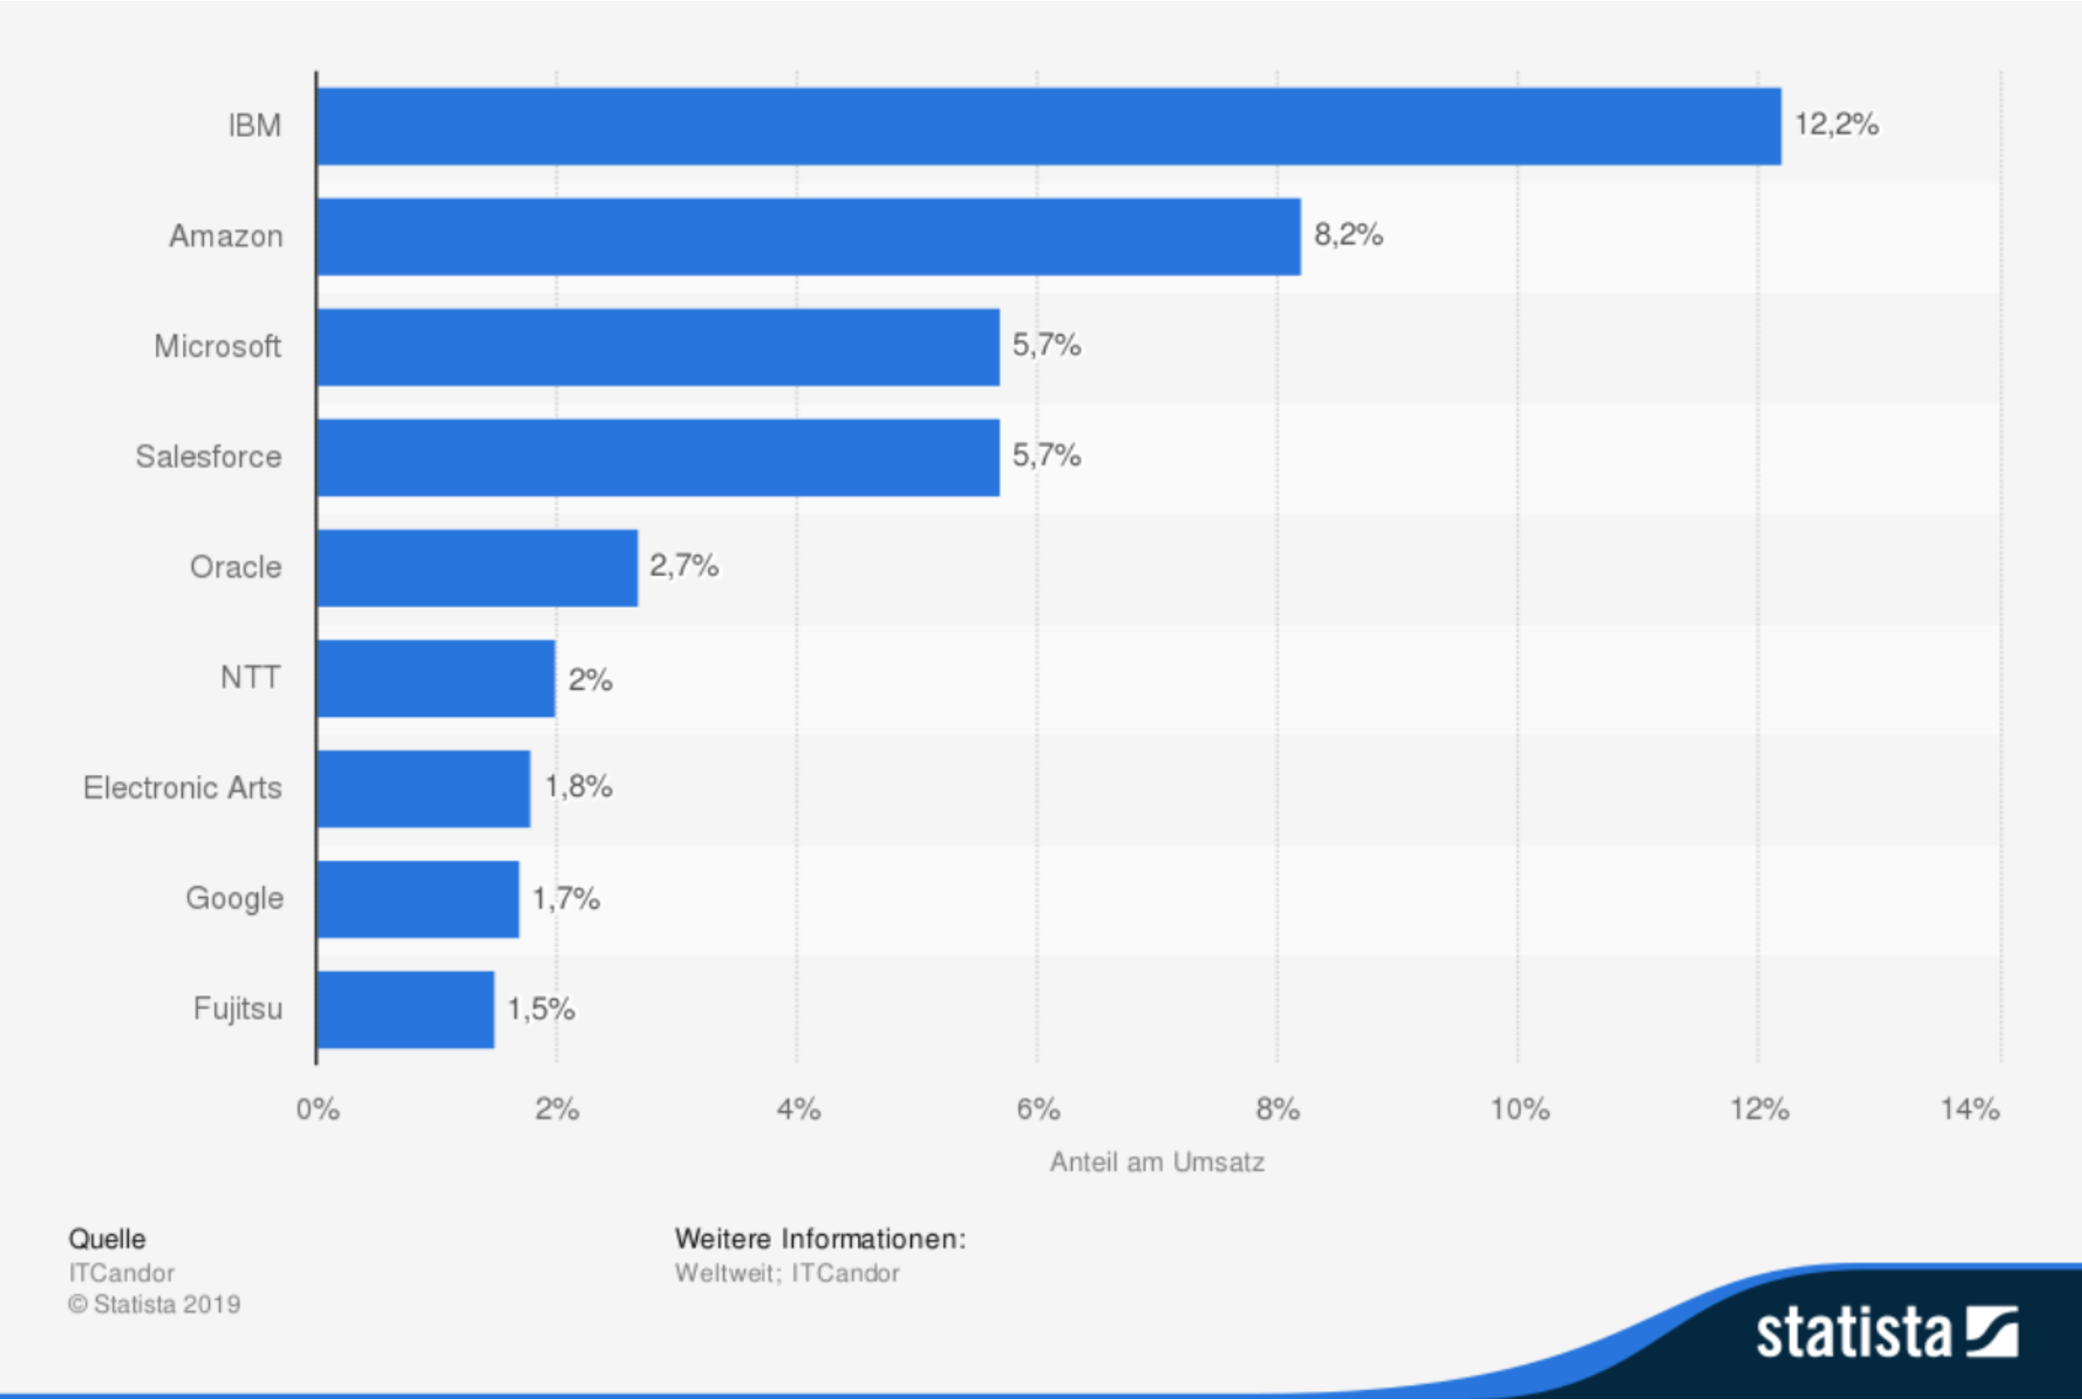
\includegraphics[scale=0.43]{img/statistic_id150979_marktanteile-der-fuehrenden-unternehmen-im-bereich-cloud-computing-weltweit-2019.pdf}
	\caption{Marktanteile der führenden Unternehmen am Umsatz im Bereich Cloud Computing weltweit von Juli 2018 bis Juni 2019}
	{\footnotesize Quelle: \cite{itcandor_cloud_2019}}
	\label{abb:marktanteileCC19}
	%		{\scriptsize \textit{Alle Rechte, einschließlich der Vervielfältigung, Veröffentlichung, Bearbeitung und Übersetzung bleiben der SV Informatik GmbH vorbehalten.}}
\end{figure}

\begin{figure}[H]
	\centering
	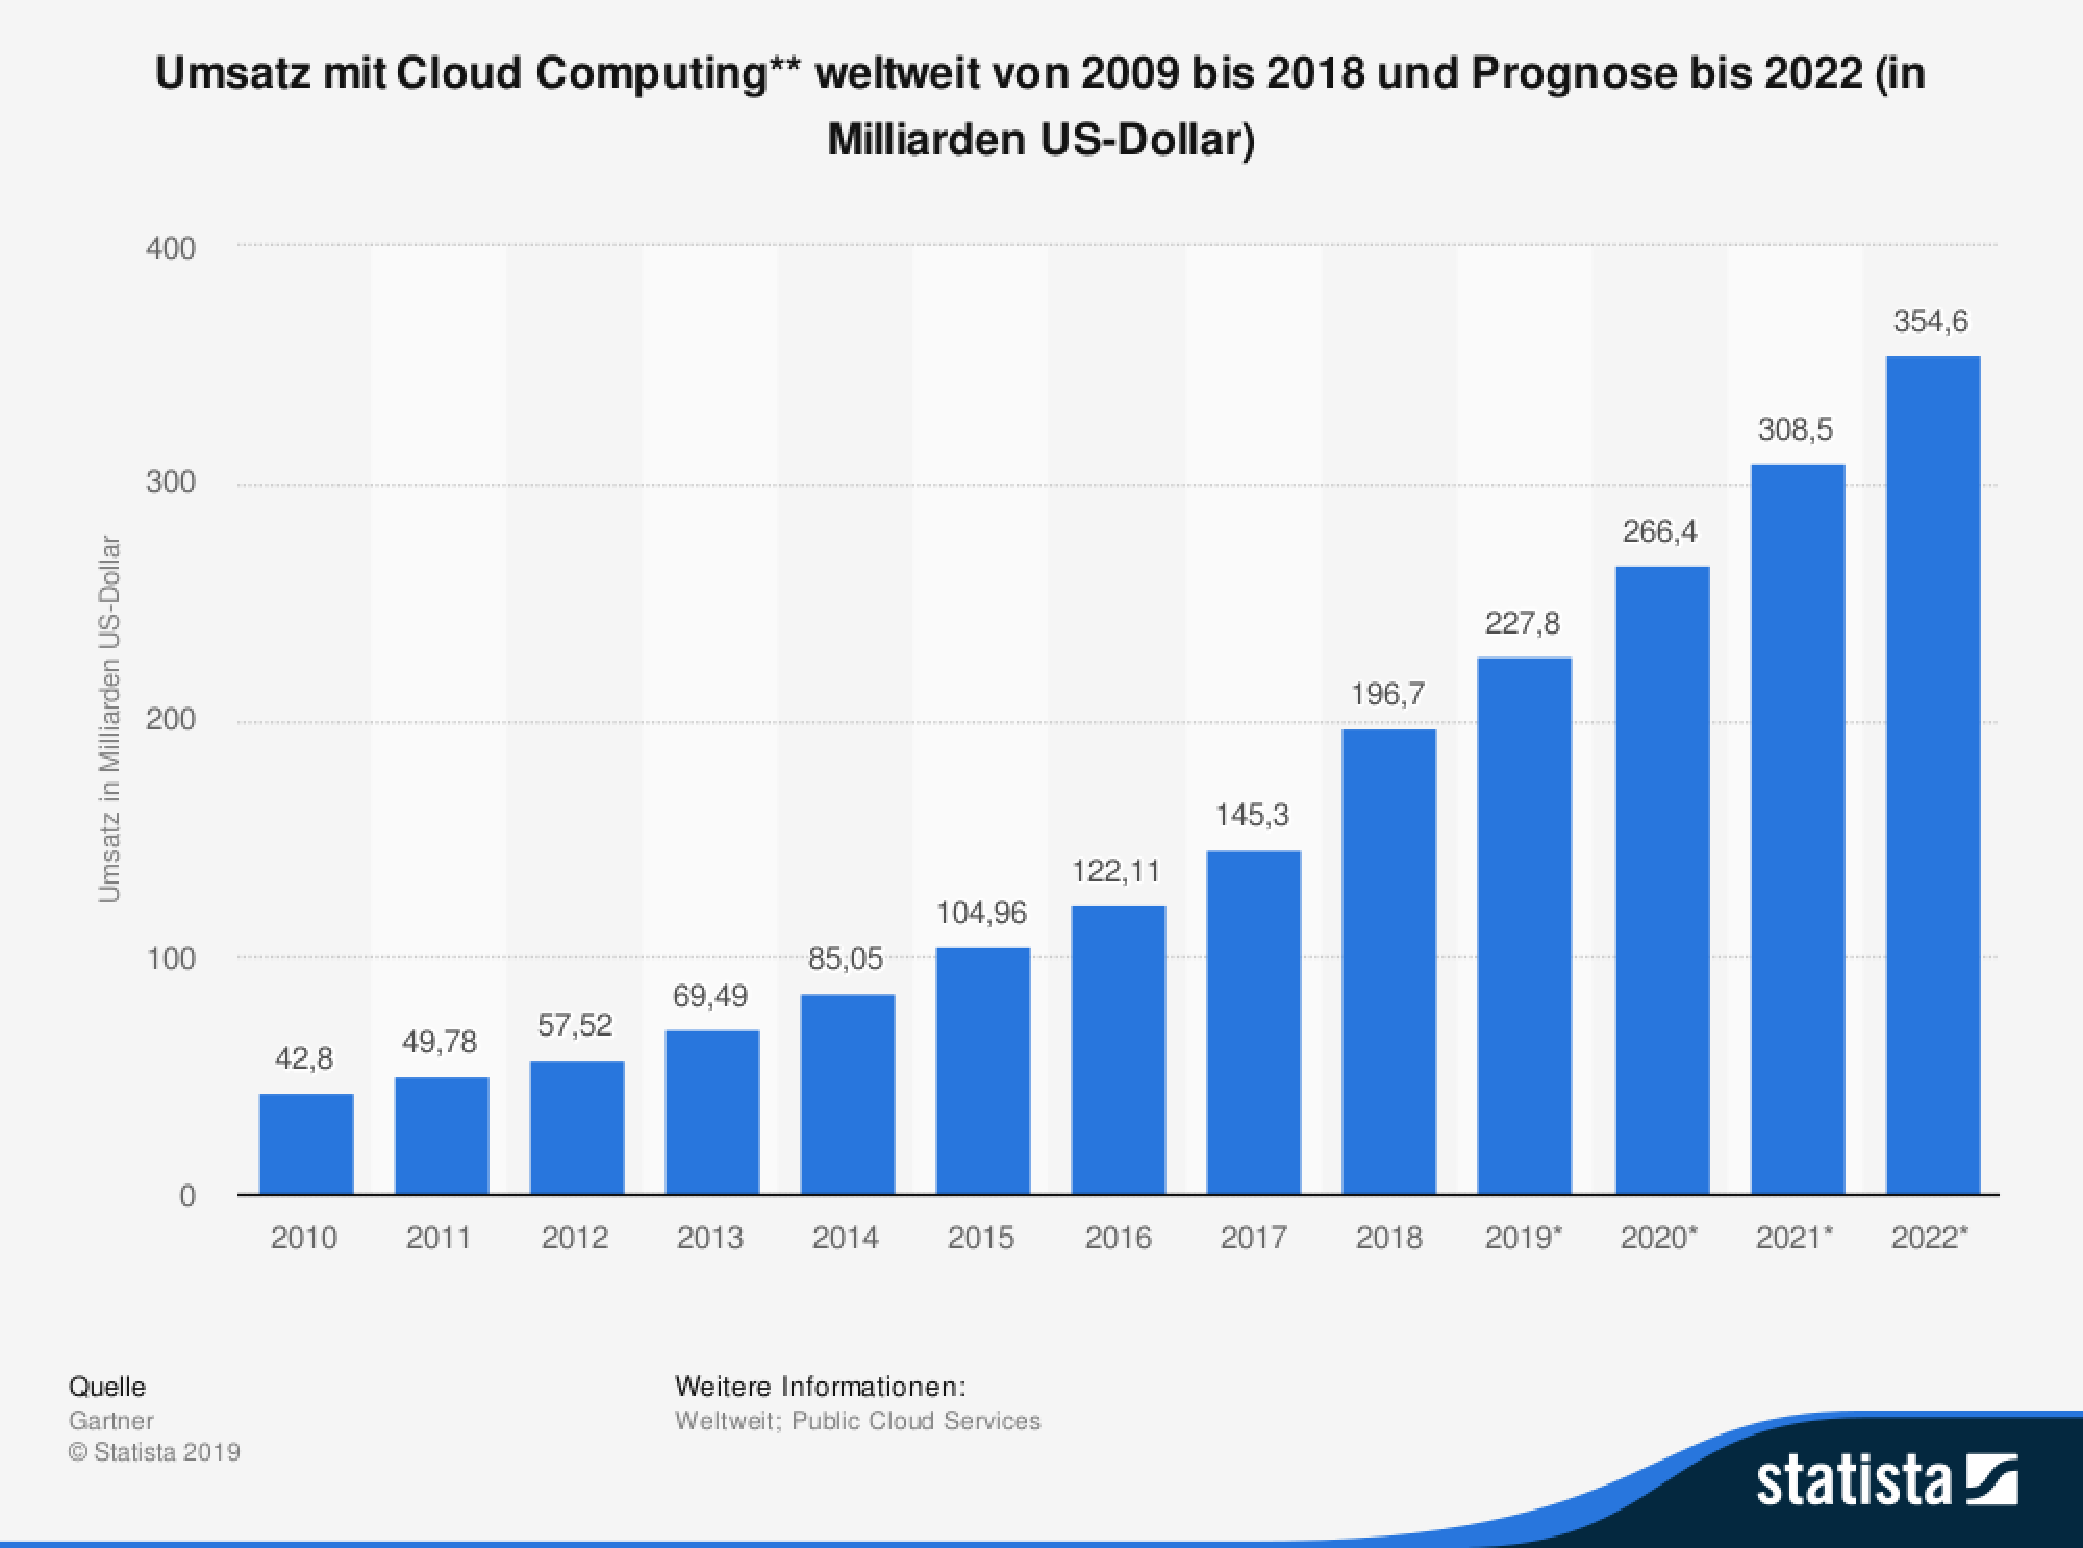
\includegraphics[scale=0.43]{img/statistic_id195760_prognose-zum-umsatz-mit-cloud-computing-weltweit-bis-2022.pdf}
	\caption{Umsatz mit Cloud-Computing weltweit von 2009 bis 2018 und Prognose bis 2022 }
	{\footnotesize Quelle: \cite{gartner_cloud_2019}}
	\label{abb:umsatzprognoseCC}
	%		{\scriptsize \textit{Alle Rechte, einschließlich der Vervielfältigung, Veröffentlichung, Bearbeitung und Übersetzung bleiben der SV Informatik GmbH vorbehalten.}}
\end{figure}

\section{Ergänzungen zum Kapitel Container(-isierung) und Orchestrierung}

\begin{figure}[H]
	\centering
	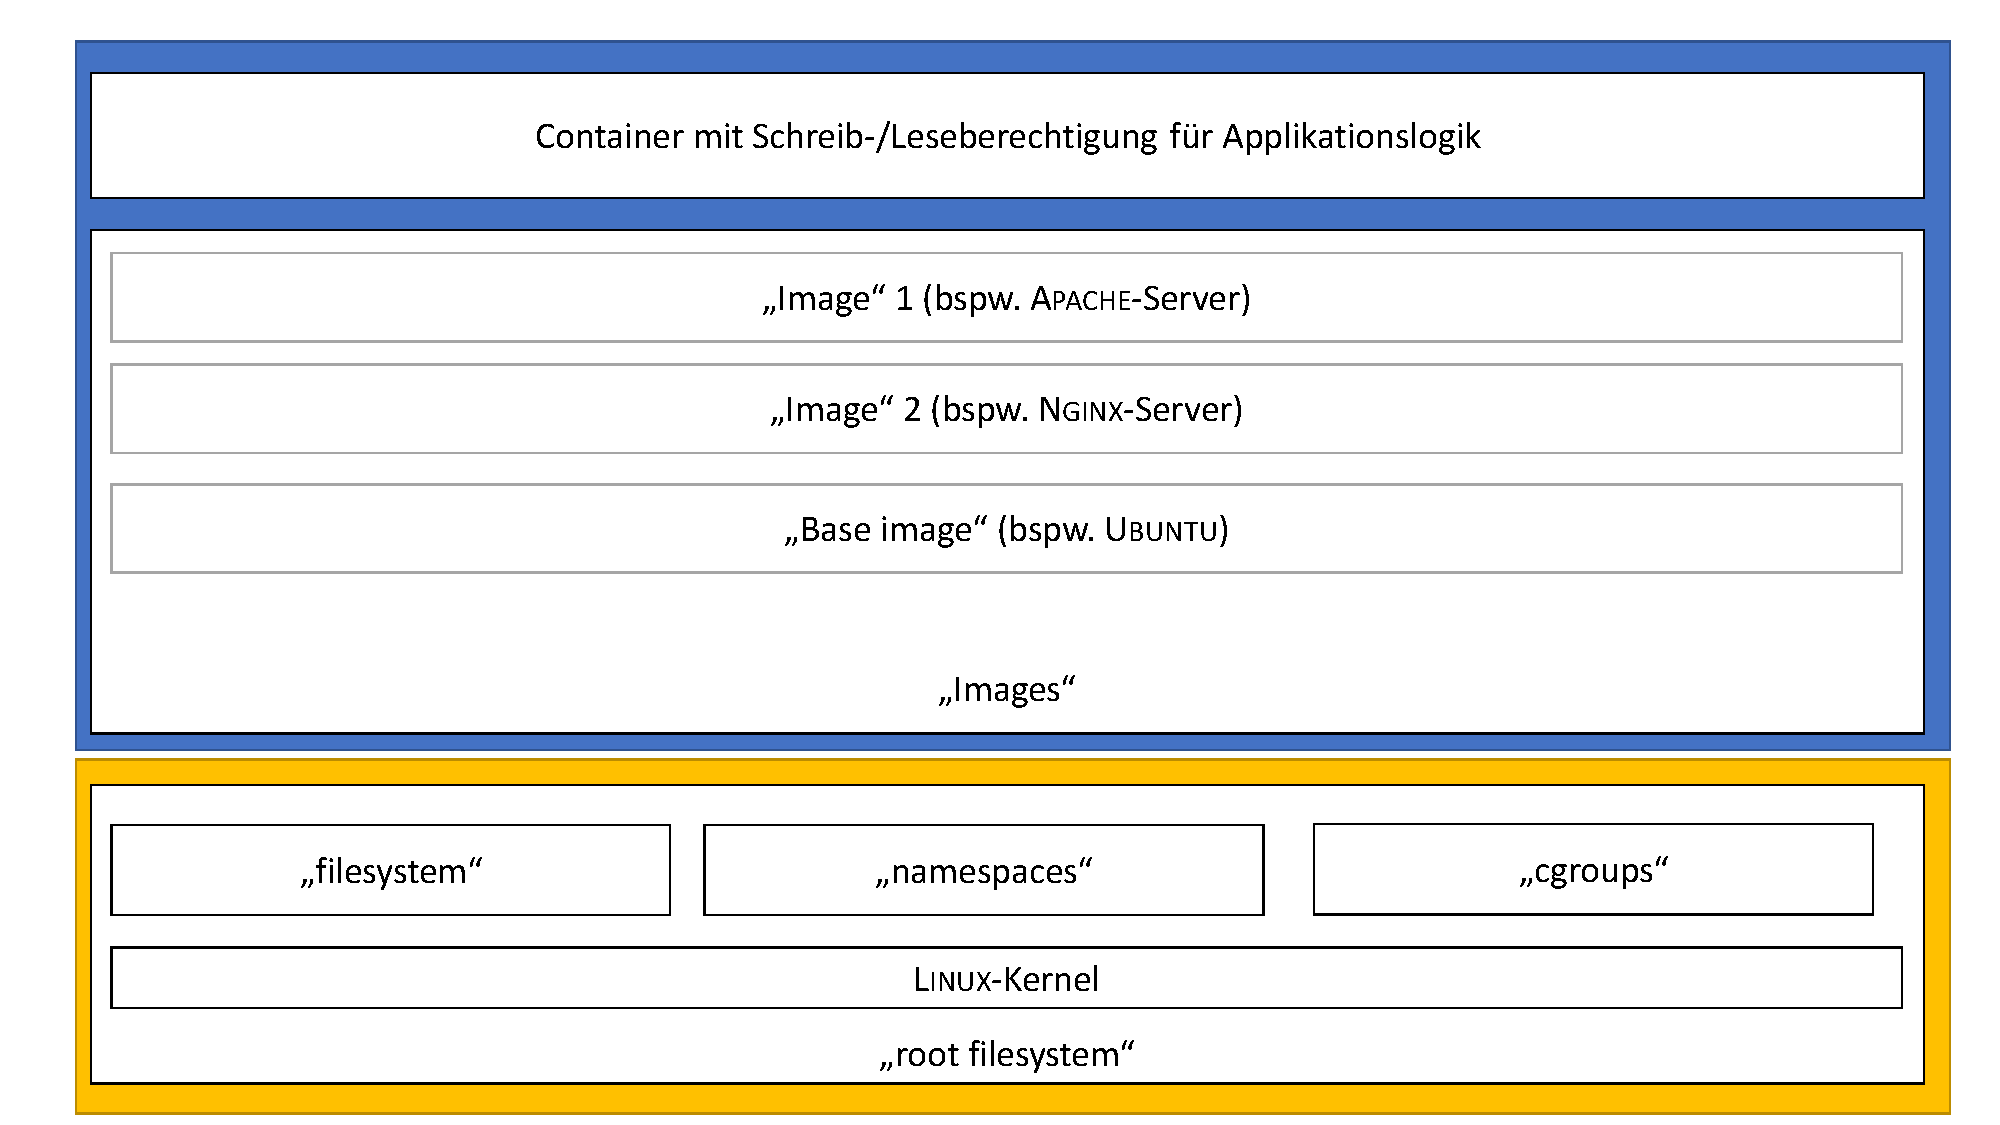
\includegraphics[scale=0.45]{img/containerImageArch.pdf}
	\caption{Architektur des Container-\enquote{Images}}
	{\footnotesize Quelle: in Anlehnung an \cite{pahl_containerization_2015}}
	\label{abb:containerArch}
	%		{\scriptsize \textit{Alle Rechte, einschließlich der Vervielfältigung, Veröffentlichung, Bearbeitung und Übersetzung bleiben der SV Informatik GmbH vorbehalten.}}
\end{figure}

Hierbei ist zu beachten, dass das orange gefärbte die Funktionalitäten der \textsc{Docker}-\enquote{Engine} und das blau gefärbte die möglichen Bestandteile eines \textsc{Docker}-\enquote{Images} darstellen soll.


\begin{figure}[H]
	\centering
	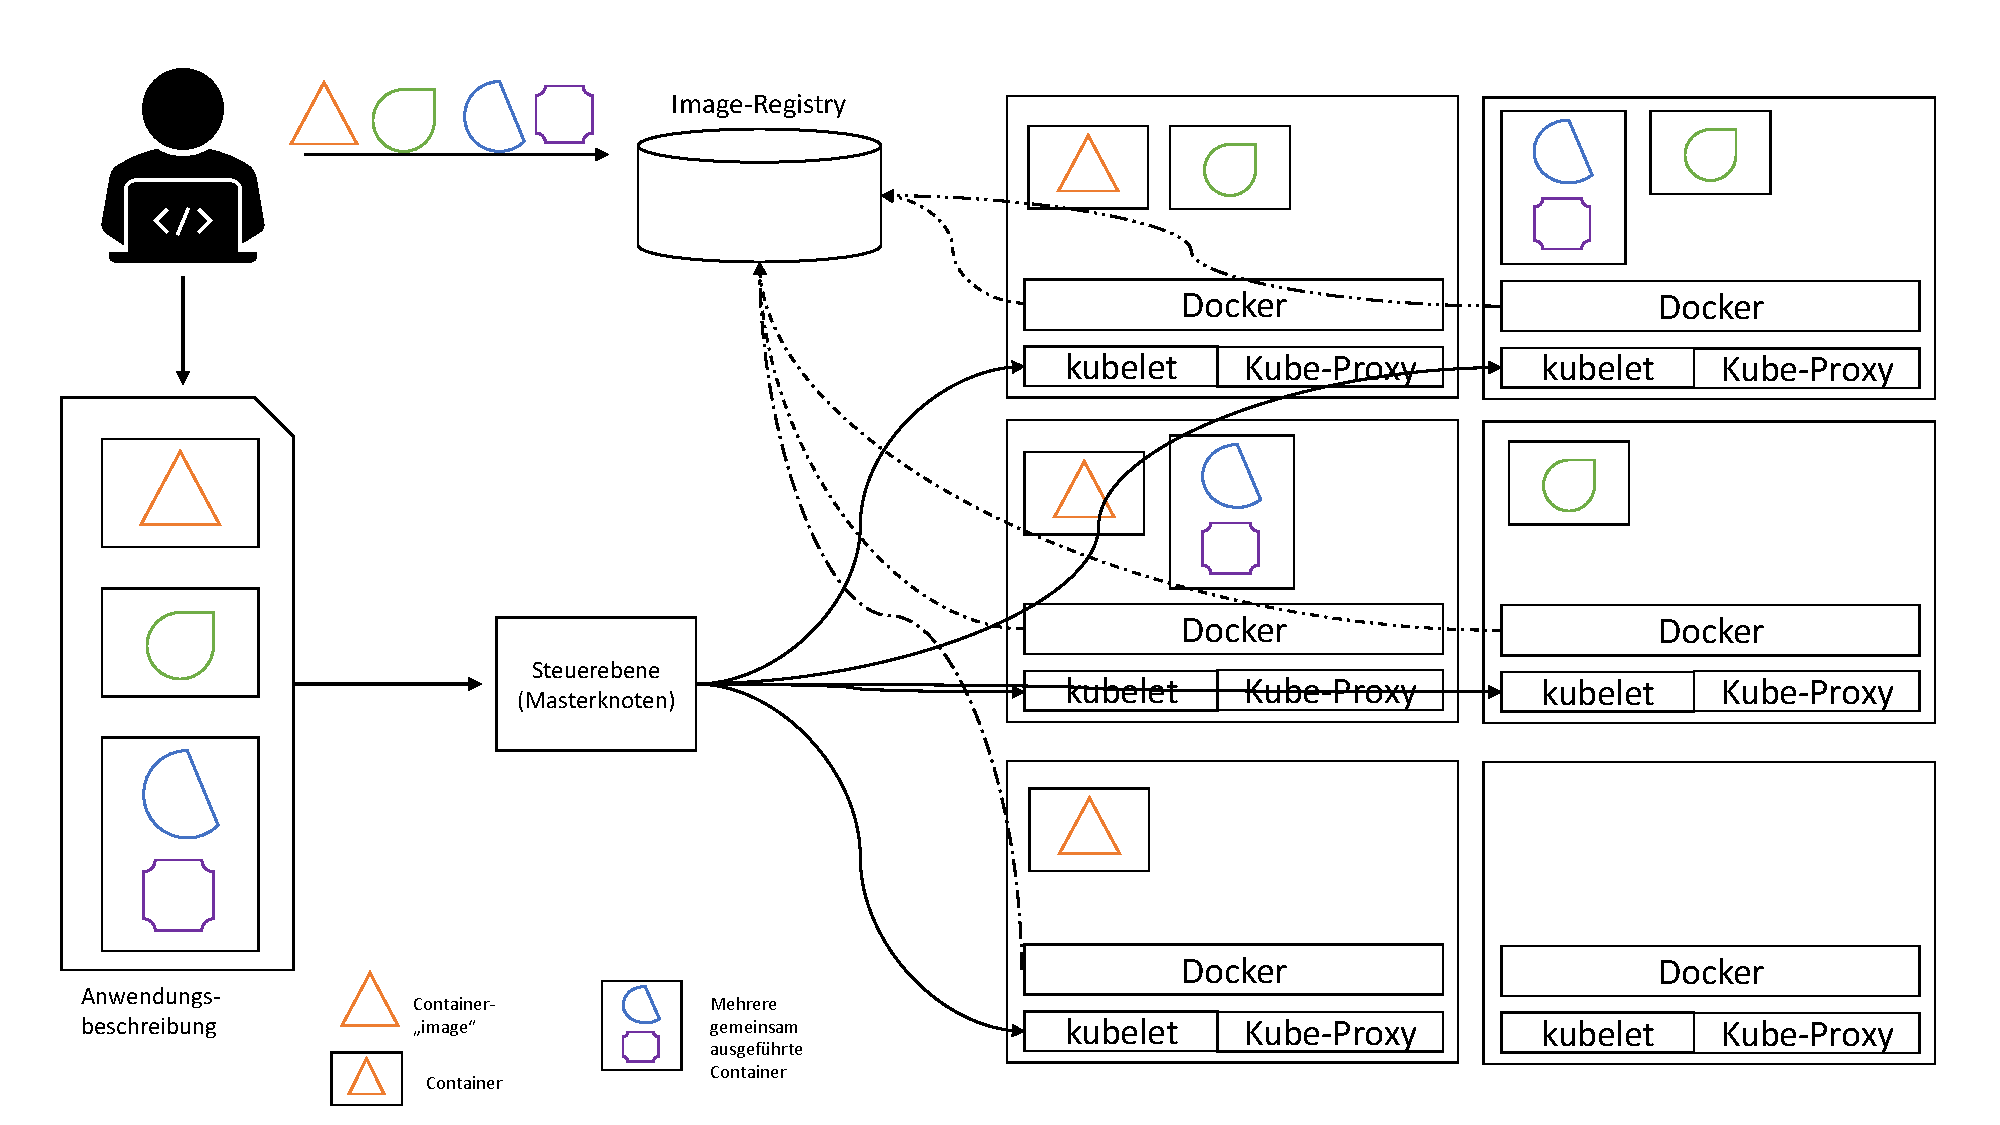
\includegraphics[scale=0.46]{img/k8sArch.pdf}
	\caption{Überblick über eine \textsc{Kubernetes}-Architektur}
	{\footnotesize Quelle: in Anlehnung an \cite[][S.\,23]{luksa_kubernetes_2018}}
	\label{abb:k8sArch}
	%		{\scriptsize \textit{Alle Rechte, einschließlich der Vervielfältigung, Veröffentlichung, Bearbeitung und Übersetzung bleiben der SV Informatik GmbH vorbehalten.}}
\end{figure}

\begin{figure}[H]
	\centering
	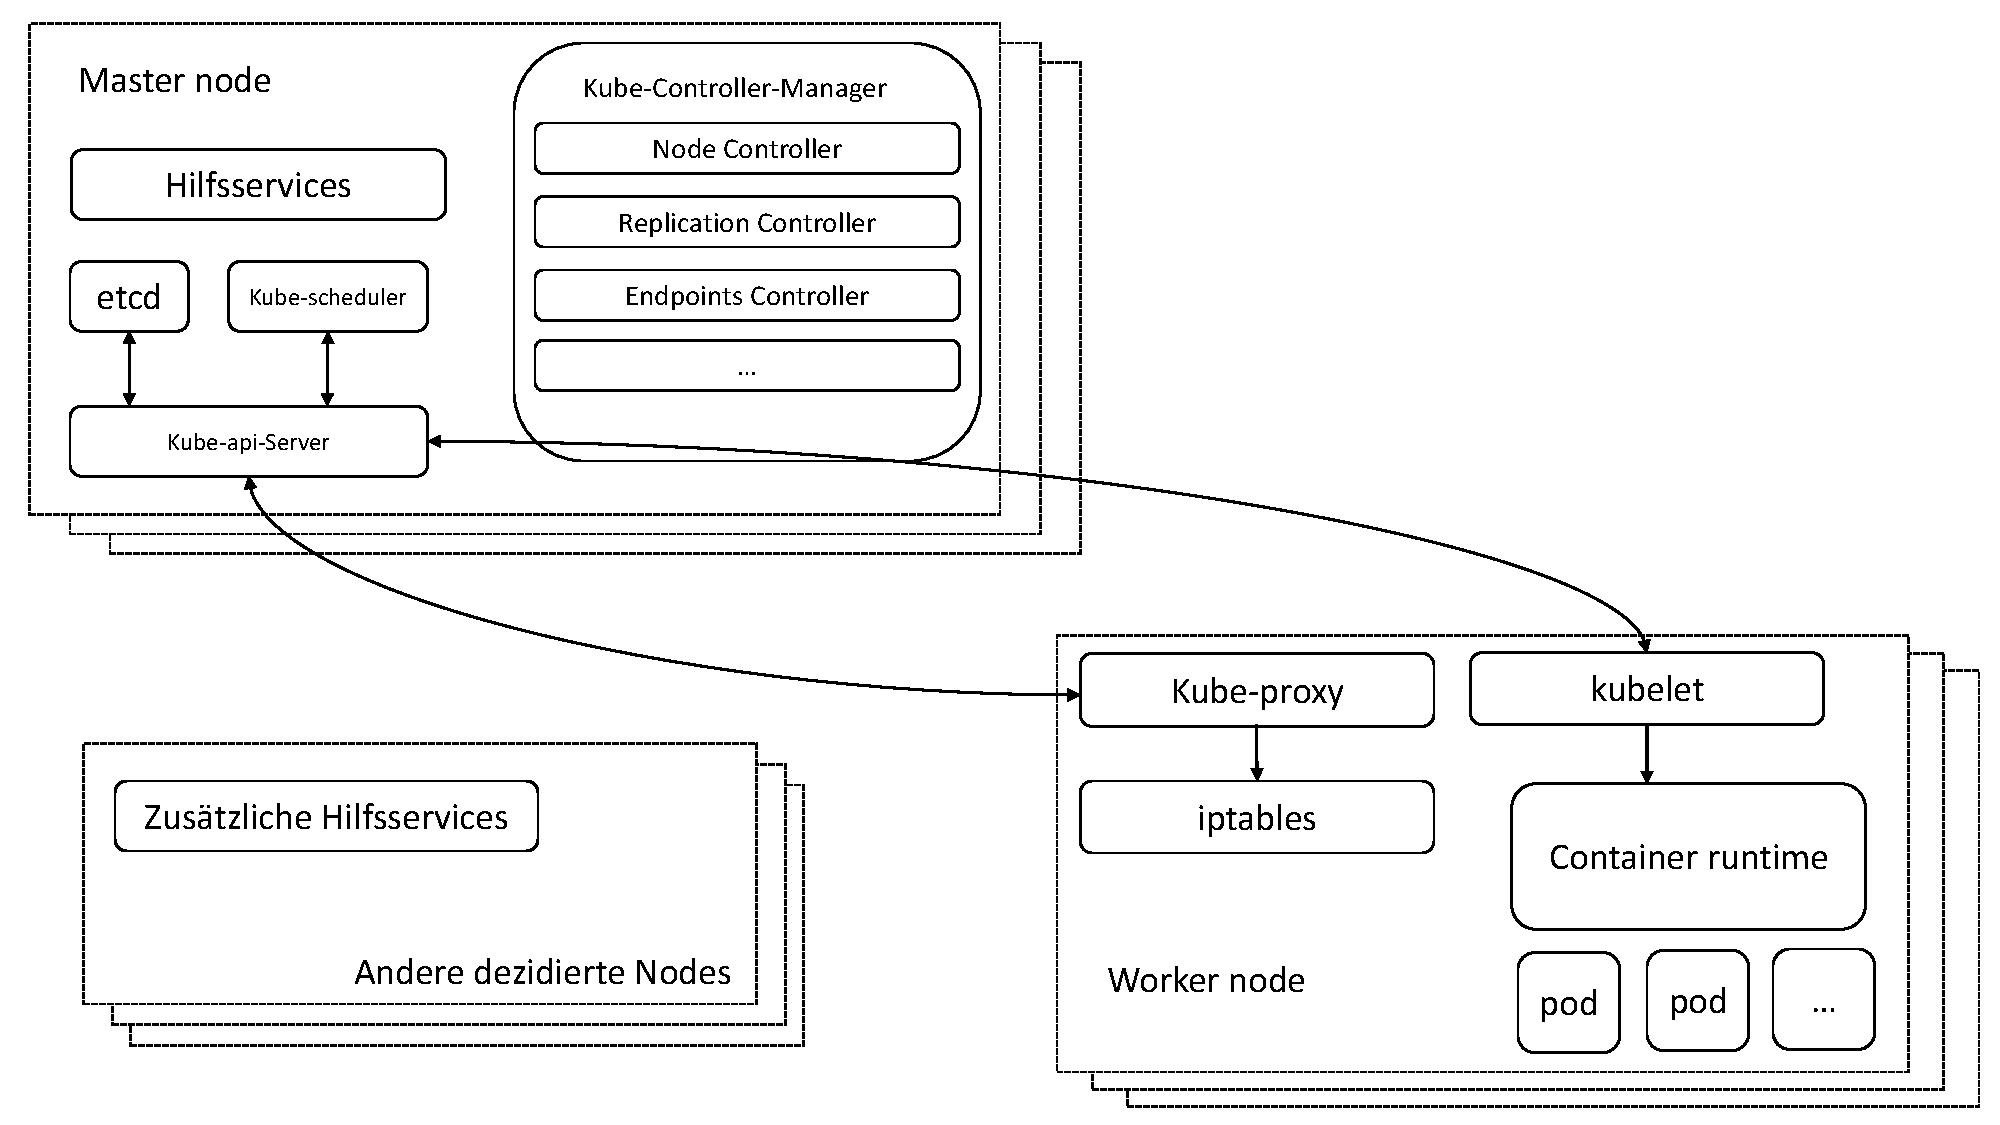
\includegraphics[scale=0.46]{img/k8sArchInteraktion.pdf}
	\caption{Architektur der \enquote{\ac{K8s}}-Interaktion}
	{\footnotesize Quelle: in Anlehnung an \cite[][S.\,15]{caban_architecting_2019}}
	\label{abb:k8sArchInteraktion}
	%		{\scriptsize \textit{Alle Rechte, einschließlich der Vervielfältigung, Veröffentlichung, Bearbeitung und Übersetzung bleiben der SV Informatik GmbH vorbehalten.}}
\end{figure}

\section{Anforderungskatalog der Forschungsfrage eins}
Die Klassifizierung beschreibt die Wichtigkeit (gering, mittel, hoch) im Kontext des
zu implementierenden Prozesses und die Nummer dient der besseren Identifizierbarkeit der jeweiligen Anforderung.
\begin{table*}[h!]
	\centering
	\ra{1.3} %more space beetween rules
	
	\begin{tabular}{@{}lp{6.5cm}l@{}}\toprule[1.5pt]
		
		\textbf{Nummer} & \textbf{Klassifizierung} & \textbf{Anforderung} \\ \midrule
		% below rules with content
		
		Test                      & Def                 & Autor           \\
		
		\bottomrule[1.5pt]
	\end{tabular}
	
	\caption{Anforderungskatalog zum implementierenden Prozess}
	\label{tab:anforderungslisteFF1}
	
\end{table*}

\clearpage

\section{Quellcode zum Testen der Webseiten-Verfügbarkeit}
% LISTING
\lstinputlisting[language=sh, caption={Funktion zum Testen, ob eine Webseite verfügbar ist}, label=lst:testConnection]{resources/listings/testConnection.sh}

\chapter{Ergänzungen zur Forschungsfrage zwei} \label{appendixFF2}
In diesem Teil des Anhangs sind Ergänzungen zur Forschungsfrage zwei des Kapitels \vref{ff2} beschrieben.

\section{Entscheidung über die Notwendigkeit eines \enquote{Business Case}}

\begin{figure}[H]
	\centering
	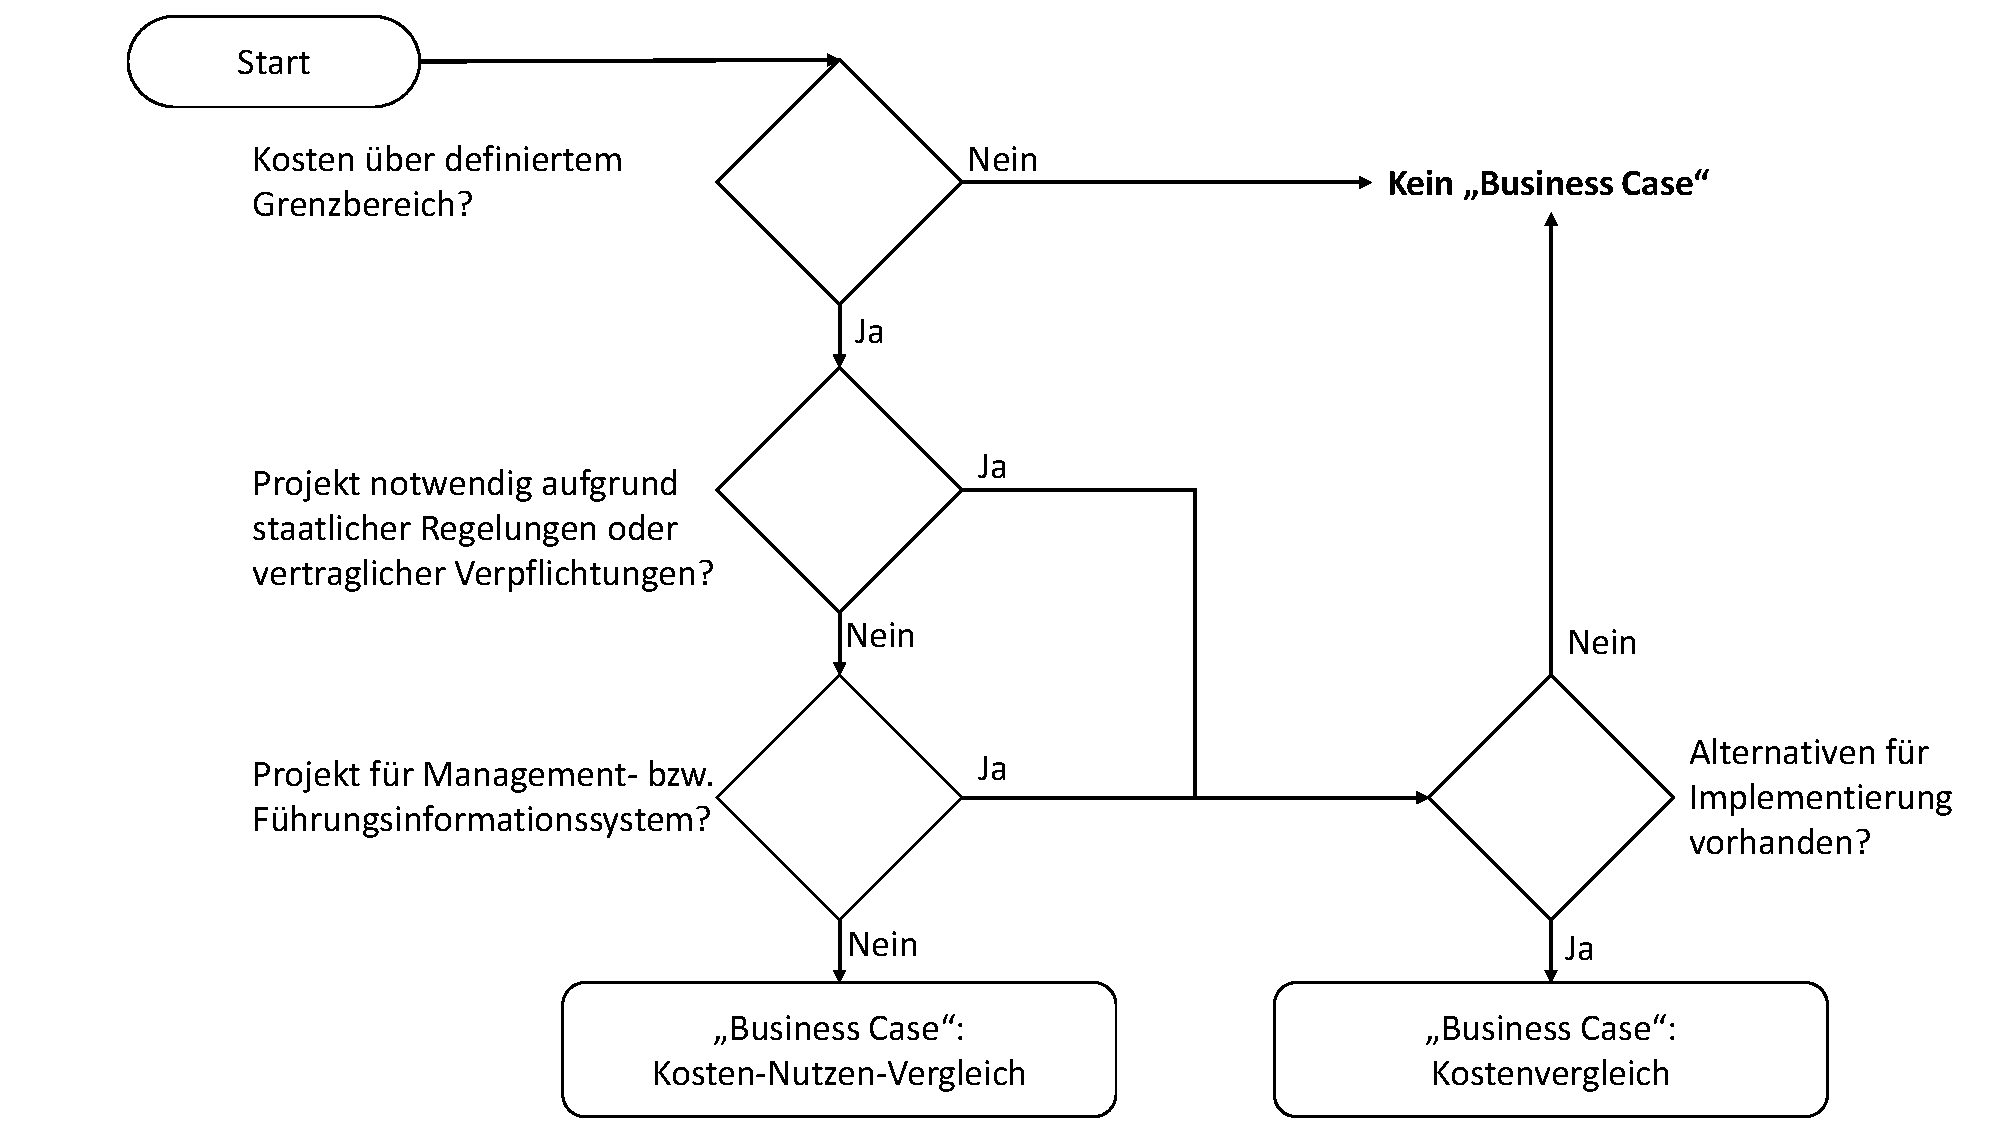
\includegraphics[scale=0.48]{img/entscheidungBC.pdf}
	\caption{Notwendigkeit eines \enquote{Business Case}}
	{\footnotesize Quelle: in Anlehnung an \cite[][S.\,29]{brugger_it_2009}}
	\label{abb:entscheidungBC}
	%		{\scriptsize \textit{Alle Rechte, einschließlich der Vervielfältigung, Veröffentlichung, Bearbeitung und Übersetzung bleiben der SV Informatik GmbH vorbehalten.}}
\end{figure}

\section{Vor-/Nachteile der internen beziehungsweise externen Erstellung eines \enquote{Business Case}}\label{appendixVorNachteileErstellungBC}

\begin{table*}[h!]
	\centering
	\ra{1.3} %more space beetween rules
	
	\begin{tabular}{@{}ll@{}}\toprule[1.5pt]
		
		\textbf{Vorteile} & \textbf{Nachteile} \\ \midrule
		
		% below rules with content
		Neutralität & Kein Wissenstransfer \\
		Verfügbarkeit & Kosten, egal ob der \enquote{Business Case} rentabel ist\\
		Effiziente Erstellung & hohe Kosten im Vergleich zur internen Erstellung \\
		Glaubwürdigkeit & Abhängigkeit \\
		Qualität & Verlust der firmeninternen Standards \\
		Innovation & \\
		Schlichtung & \\
		
		\bottomrule[1.5pt]
	\end{tabular}
	
	\caption{Überblick über die Vor-/Nachteile der externen Erstellung eines \enquote{Business Case}}
	{\footnotesize Quelle: in Anlehnung an \cite[][S.\,34]{brugger_it_2009}}
	\label{tab:externVorNachteile}
	
\end{table*}

\begin{table*}[h!]
	\centering
	\ra{1.3} %more space beetween rules
	
	\begin{tabular}{@{}ll@{}}\toprule[1.5pt]
		
		\textbf{Vorteile} & \textbf{Nachteile} \\ \midrule
		
		% below rules with content
		Wissensaufbau & Verfügbarkeit \\
		Qualität & Effizienzverlust bei rein technischen/operativen Mitarbeitern \\
		\enquote{Teamwork} & Glaubwürdigkeit \\
		Standardisierung & Qualitätskontrolle durch \enquote{Controlling}-Division \\
		
		\bottomrule[1.5pt]
	\end{tabular}
	
	\caption{Überblick über die Vor-/Nachteile der internen Erstellung eines \enquote{Business Case}}
	{\footnotesize Quelle: in Anlehnung an \cite[][S.\,34]{brugger_it_2009}}
	\label{tab:internVorNachteile}
	
\end{table*}

\begin{figure}[H]
	\centering
	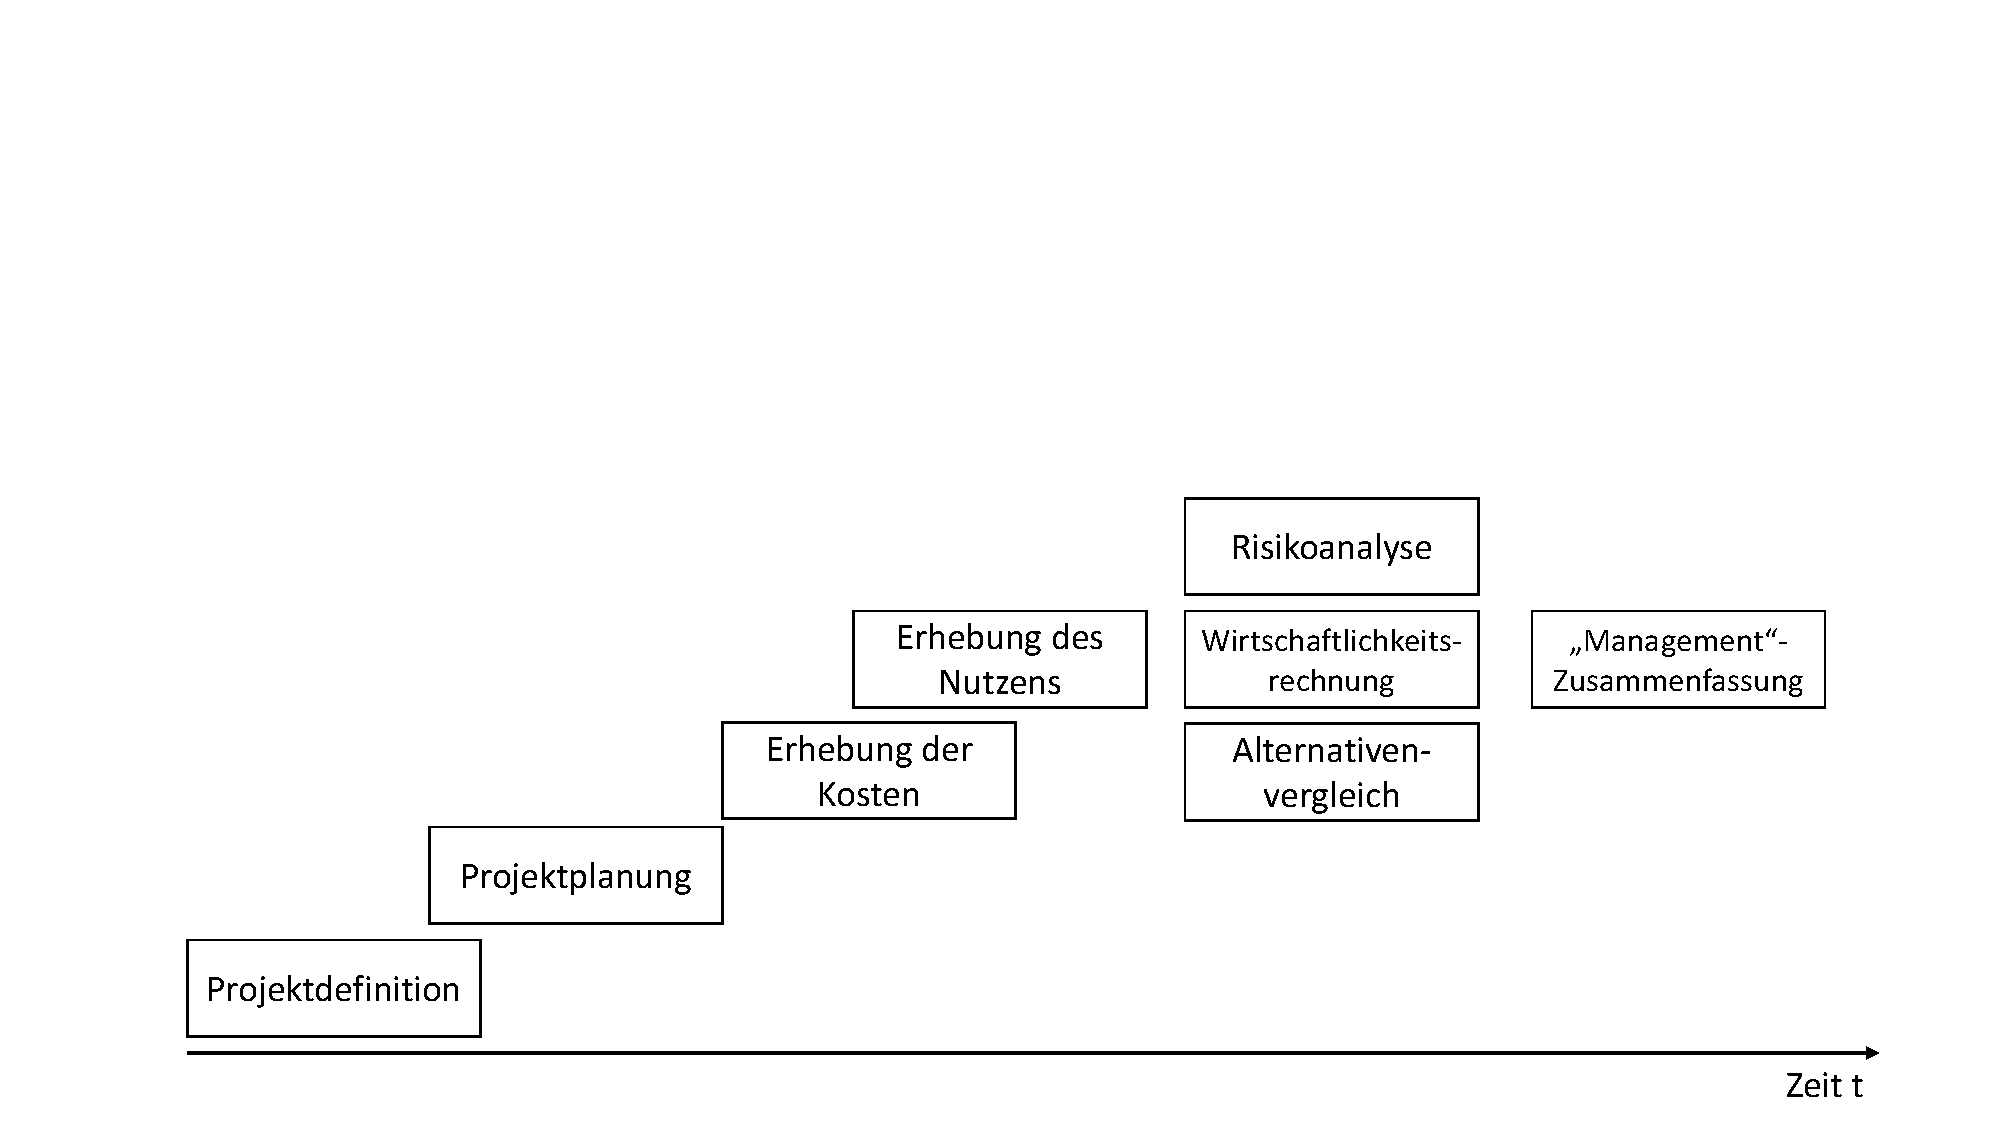
\includegraphics[scale=0.48]{img/chronoBC.pdf}
	\caption{Chronologische Abfolge der Entwicklungsphase eines \enquote{Business Case}}
	{\footnotesize Quelle: in Anlehnung an \cite[][]{herman_is_2009}}
	\label{abb:entwicklungBC}
	%		{\scriptsize \textit{Alle Rechte, einschließlich der Vervielfältigung, Veröffentlichung, Bearbeitung und Übersetzung bleiben der SV Informatik GmbH vorbehalten.}}
\end{figure}

\chapter{Ergänzungen zur Forschungsfrage drei} \label{appendixFF3}
In diesem Teil des Anhangs sind Ergänzungen zur Forschungsfrage drei des Kapitels \vref{ff3} beschrieben.

\section{\enquote{Plan-Do-Check-Act}-Regelkreis}

\begin{figure}[H]
	\centering
	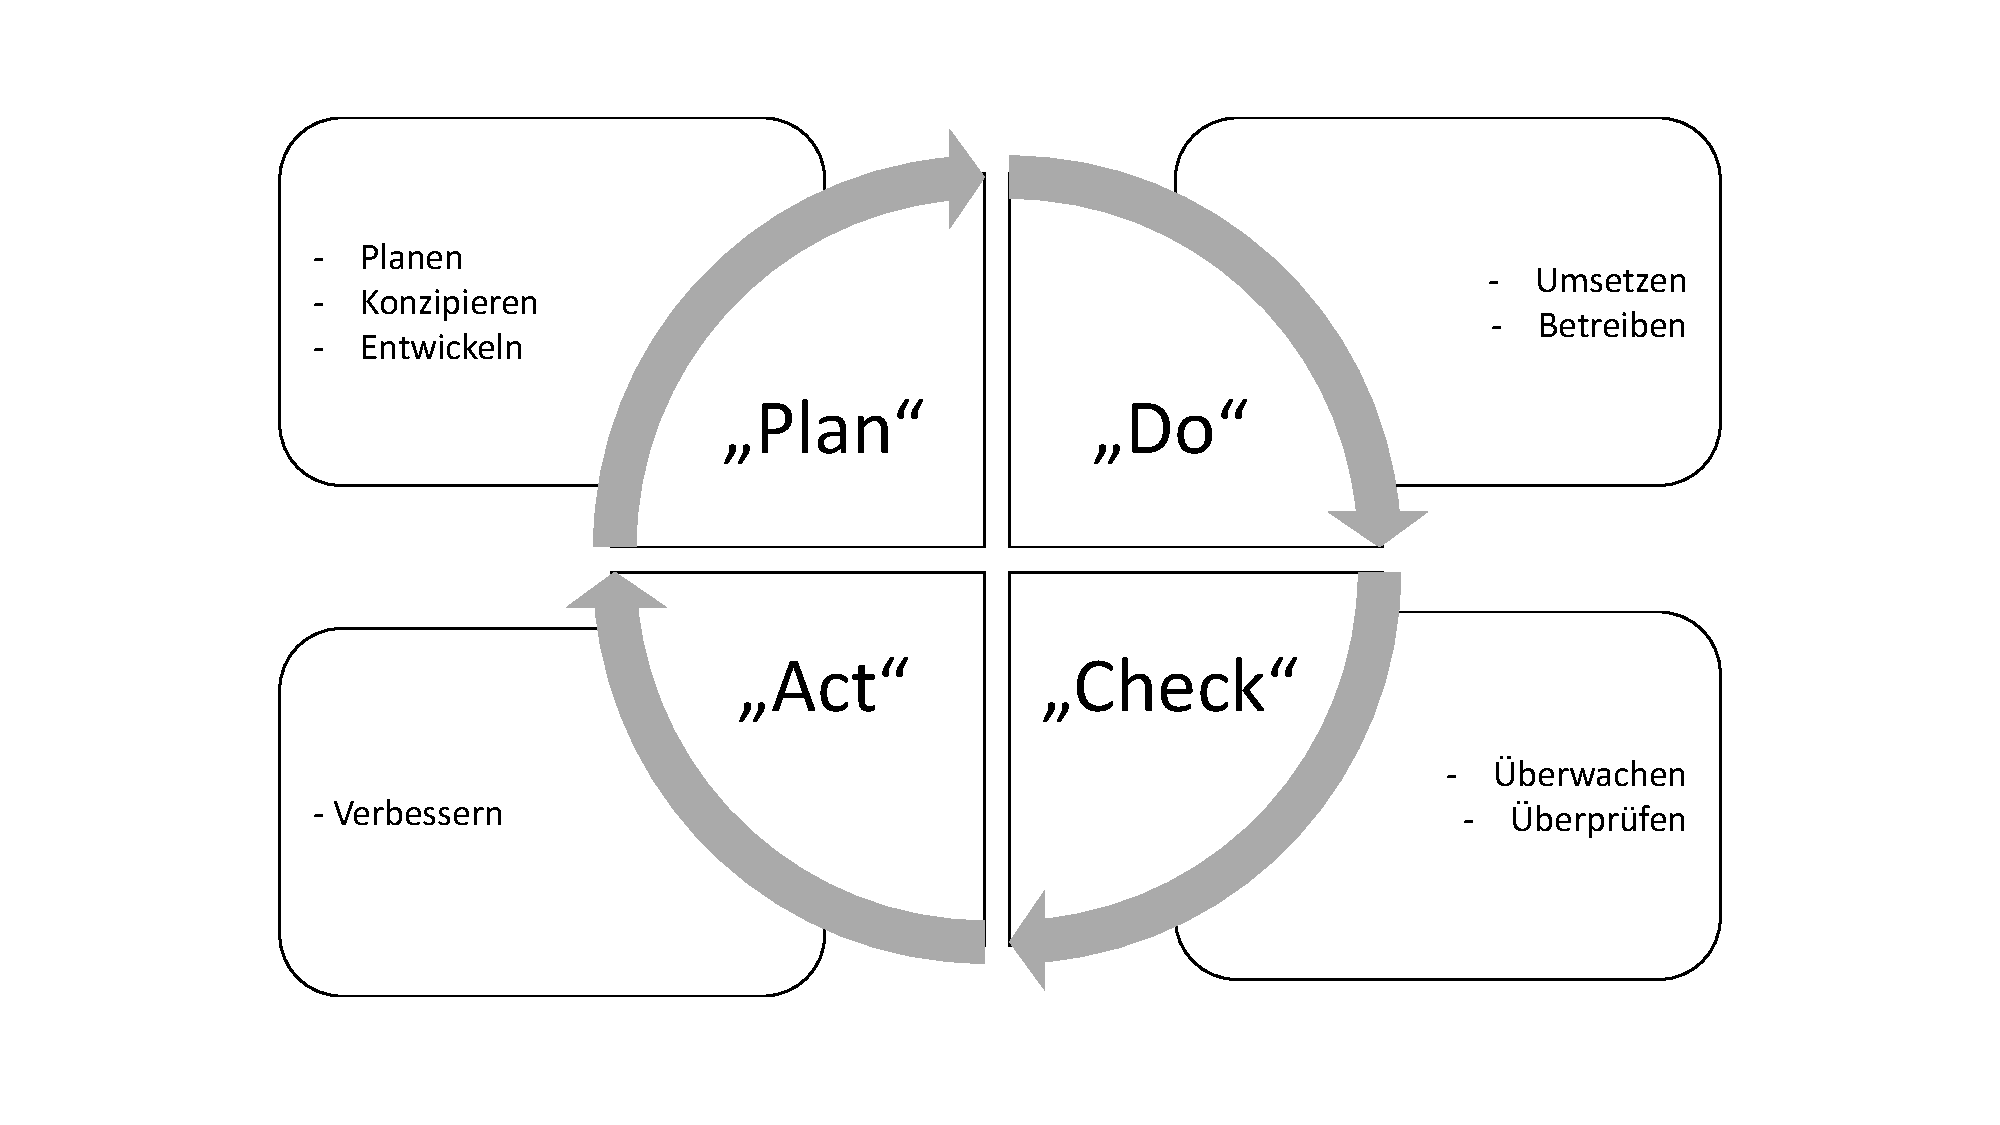
\includegraphics[scale=0.51]{img/planDoCheckAct.pdf}
	\caption{Der \enquote{Plan-Do-Check-Act}-Regelkreis}
	{\footnotesize Quelle: in Anlehnung an \cite[][S.\,12]{kersten_it-sicherheitsmanagement_2020}}
	\label{abb:planDoCheckAct}
	%		{\scriptsize \textit{Alle Rechte, einschließlich der Vervielfältigung, Veröffentlichung, Bearbeitung und Übersetzung bleiben der SV Informatik GmbH vorbehalten.}}
\end{figure}

\clearpage % neue Seite
\section{Checkliste zur Vorbereitung der \ac{ISMS}-Einführung}
\begin{table*}[h!]
	\centering
	\ra{1.3} %more space beetween rules
	
	\begin{tabular}{@{}lp{10cm}l@{}}\toprule[1.5pt]
		
		\textbf{Aktion} & \textbf{Gegenstand} & \textbf{Erfüllt?} \\ \midrule
		% below rules with content
		
		1 & Sind die Normen (27000, 27001, 27002) in aktueller elektronischer
		Form vorhanden? & $\square$ \\
		2 & Sind die Vorteile und der Nutzen eines ISMS erläutert worden? & $\square$ \\
		3 & Ist ein Grob-Abgleich mit ISO 27001 erfolgt? (Ziel: erste
		Aufwandsabschätzung) & $\square$ \\
		4 & Ist eine Entscheidung zur Orientierung an der ISO 27001
		getroffen worden? & $\square$ \\
		5 & Denken wir in Management-Systemen? Existieren schon andere
		Management-Systeme? & $\square$ \\
		6 & Ist der Begriff ISMS eingeführt? & $\square$ \\
		7 & Denken wir in Geschäftsprozessen und informationstechnischen Anwendungen? & $\square$ \\
		8 & Ist der Anwendungsbereich des ISMS (Scope) zumindest grob
		skizziert? & $\square$ \\
		9 & Sind zumindest die Top Level Assets und deren Asset/Risk
		Owner erfasst worden? & $\square$ \\
		10 & Wurden – zumindest grob – Sicherheitsziele für diese Assets
		festgelegt? & $\square$ \\
				
		\bottomrule[1.5pt]
	\end{tabular}
	
	\caption{Checkliste zur Vorbereitung der \ac{ISMS}-Einführung}
	{\footnotesize{Quelle: in Anlehnung an \cite[][S.\,15]{kersten_it-sicherheitsmanagement_2020}}}
	\label{tab:checklisteVorbereitungISMS}
	
\end{table*}

\clearpage
\section{Schichtenmodell des IT-Grundschutzes}
\begin{figure}[H]
	\centering
	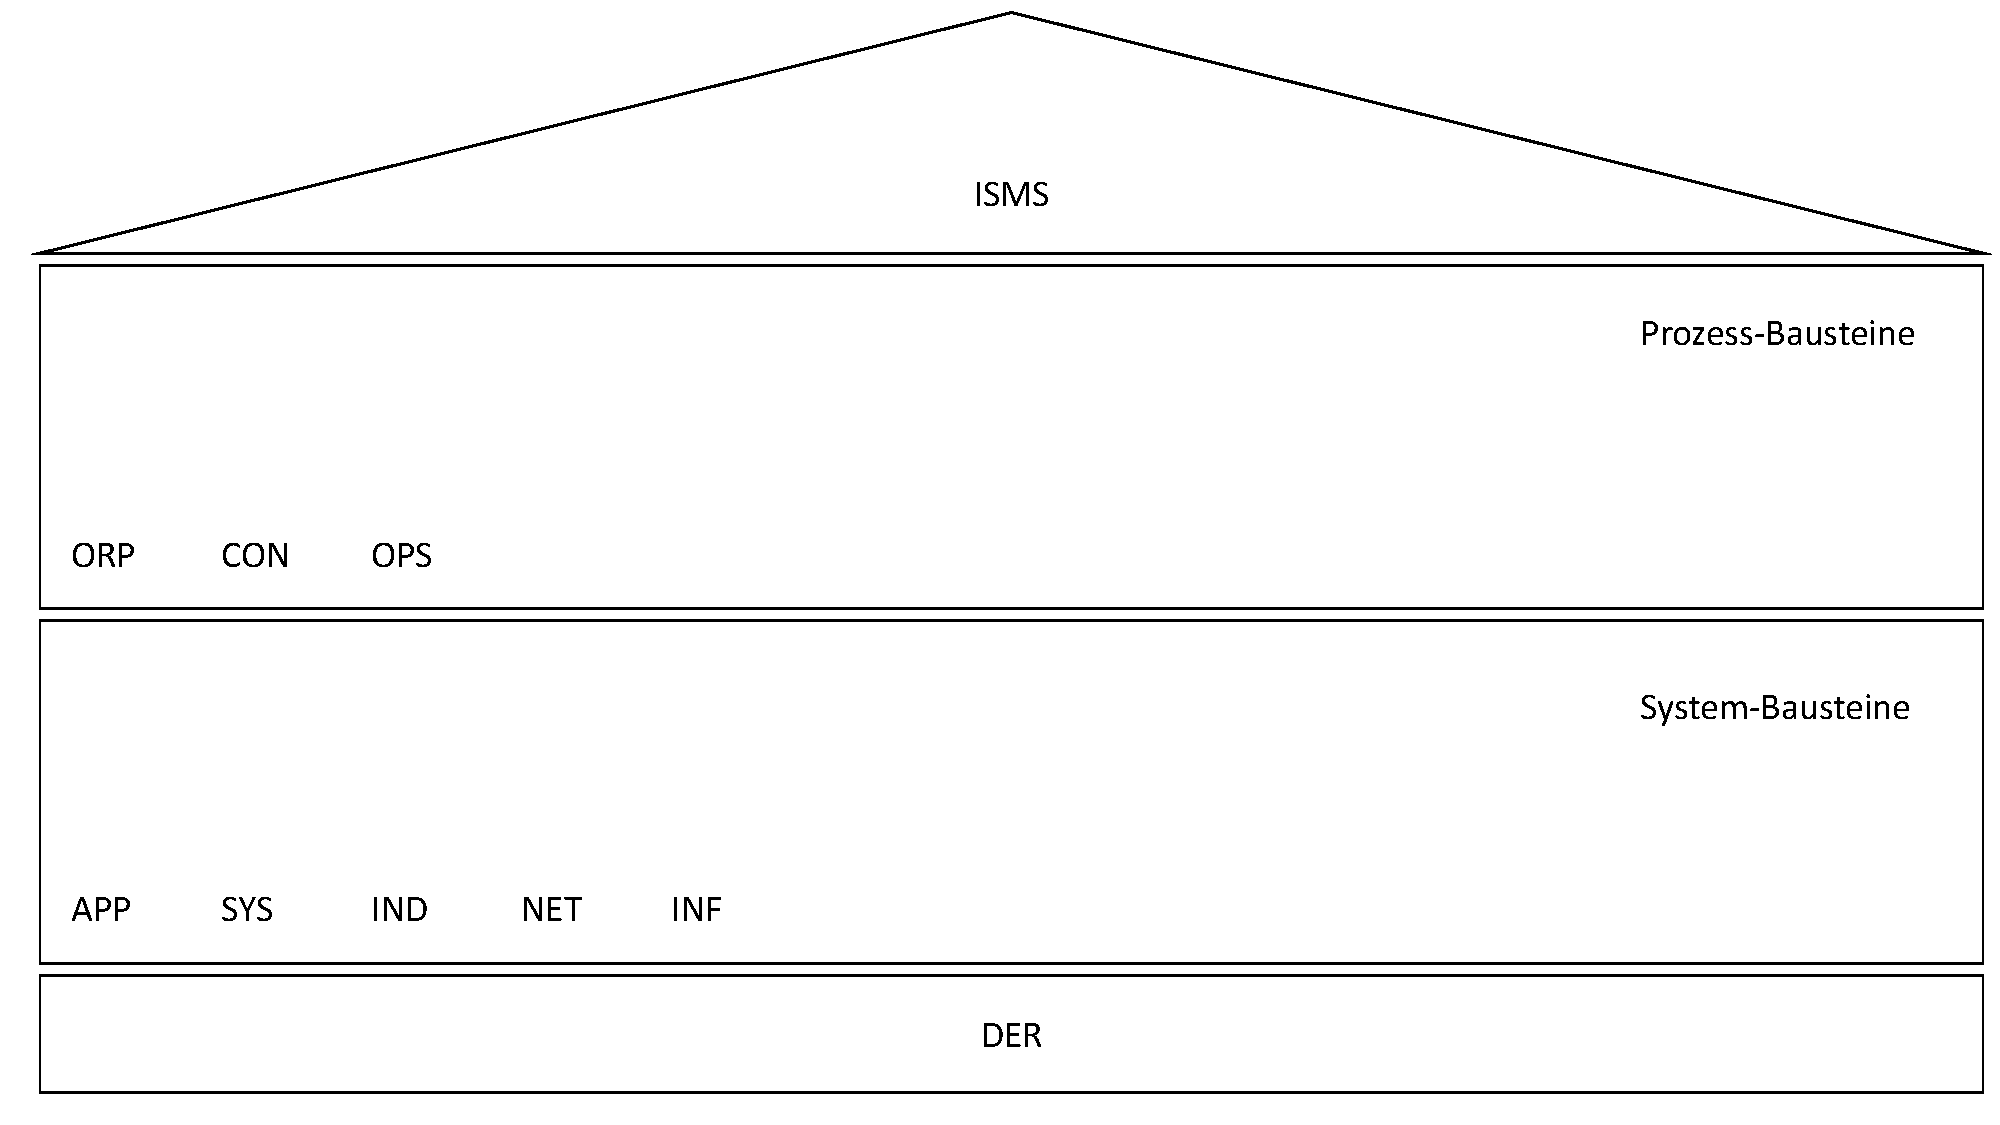
\includegraphics[scale=0.45]{img/bsiSchichtenmodell.pdf}
	\caption{Das Schichtenmodell des IT-Grundschutzes}
	{\footnotesize Quelle: in Anlehnung an \cite[][S.\,9]{bundesamt_fur_sicherheit_in_der_informationstechnik_bsi_it-grundschutz-kompendium_2020}}
	\label{abb:BSISchichtenmodell}
	%		{\scriptsize \textit{Alle Rechte, einschließlich der Vervielfältigung, Veröffentlichung, Bearbeitung und Übersetzung bleiben der SV Informatik GmbH vorbehalten.}}
\end{figure}

\enquote{Die Prozessbausteine, die in der Regel für sämtliche oder große Teile eines Informationsverbunds gleichermaßen
gelten, unterteilen sich in die folgenden Schichten, die wiederum aus weiteren Teilschichten bestehen können.
\begin{itemize}
	\item Die Schicht ISMS enthält als Grundlage für alle weiteren Aktivitäten im Sicherheitsprozess den Baustein Sicherheitsmanagement.
	\item Die Schicht ORP befasst sich mit organisatorischen und personellen Sicherheitsaspekten. In diese Schicht fallen beispielsweise die Bausteine Organisation und Personal.
	\item Die Schicht CON enthält Bausteine, die sich mit Konzepten und Vorgehensweisen befassen. Typische Bausteine
	der Schicht CON sind unter anderem Kryptokonzept und Datenschutz.
	\item Die Schicht OPS umfasst alle Sicherheitsaspekte betrieblicher Art. Insbesondere sind dies die Sicherheitsaspekte des operativen IT-Betriebs, sowohl bei einem Betrieb im Haus, als auch bei einem IT-Betrieb, der in Teilen oder komplett durch Dritte betrieben wird. Ebenso enthält er die Sicherheitsaspekte, die bei einem IT-Betrieb für Dritte zu beachten sind. Beispiele für die Schicht OPS sind die Bausteine Schutz vor Schadprogrammen und Outsourcing für Kunden.
	\item In der Schicht DER finden sich alle Bausteine, die für die Überprüfung der umgesetzten Sicherheitsmaßnahmen, die Detektion von Sicherheitsvorfällen sowie die geeigneten Reaktionen darauf relevant sind. Typische Bausteine der Schicht DER sind Behandlung von Sicherheitsvorfällen und Vorsorge für IT-Forensik.
\end{itemize}
Neben den Prozess-Bausteinen beinhaltet das IT-Grundschutz-Kompendium auch System-Bausteine. Diese werden
in der Regel auf einzelne Zielobjekte oder Gruppen von Zielobjekten angewendet. Die System-Bausteine unterteilen sich in die folgenden Schichten. Ähnlich wie die Prozess-Bausteine können auch die System-Bausteine aus weiteren Teilschichten bestehen.

\begin{itemize}
	\item Die Schicht APP beschäftigt sich mit der Absicherung von Anwendungen und Diensten, unter anderem in den
	Bereichen Kommunikation, Verzeichnisdienste, netzbasierte Dienste sowie Business- und Client-Anwendungen.
	Typische Bausteine der Schicht APP sind Allgemeine Groupware, Office-Produkte, Webserver und Relationale
	Datenbanksysteme.
	\item Die Schicht SYS betrifft die einzelnen IT-Systeme des Informationsverbunds, die ggf. in Gruppen zusammengefasst wurden. Hier werden die Sicherheitsaspekte von Servern, Desktop-Systemen, Mobile Devices und sonstigen IT-Systemen wie Druckern und TK-Anlagen behandelt. Zur Schicht SYS gehören beispielsweise Bausteine zu
	konkreten Betriebssystemen, Allgemeine Smartphones und Tablets sowie Drucker, Kopierer und Multifunktionsgeräte.
	\item Die Schicht IND befasst sich mit Sicherheitsaspekten industrieller IT. In diese Schicht fallen beispielsweise die Bausteine Betriebs- und Steuerungstechnik, Allgemeine ICS-Komponente und Speicherprogrammierbare Steuerung (SPS).
	\item Die Schicht NET betrachtet die Vernetzungsaspekte, die sich nicht primär auf bestimmte IT-Systeme, sondern
	auf die Netzverbindungen und die Kommunikation beziehen. Dazu gehören zum Beispiel die Bausteine NetzManagement, Firewall und WLAN-Betrieb.
	\item Die Schicht INF befasst sich mit den baulich-technischen Gegebenheiten, hier werden Aspekte der infrastrukturellen Sicherheit zusammengeführt. Dies betrifft unter anderem die Bausteine Allgemeines Gebäude und Rechenzentrum.
\end{itemize}}\autocite[][S.\,23-24]{bundesamt_fur_sicherheit_in_der_informationstechnik_bsi_it-grundschutz-kompendium_2020}


